\documentclass{standalone}
\usepackage{tikz, tikz-cd}
\usetikzlibrary{shapes, decorations.markings}
\begin{document}

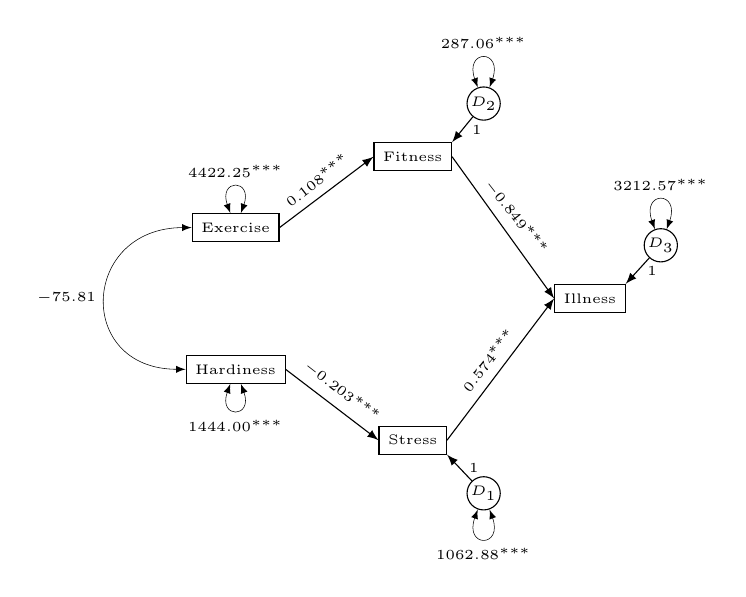
\begin{tikzpicture}[scale=0.9]
\node[draw] (y1) at (6,4) {\tiny{Illness}};
\node[draw] (x1) at (1,3) {\tiny{Hardiness}};
\node[draw] (x2) at (1,5) {\tiny{Exercise}};
\node[draw] (m1) at (3.5,2) {\tiny{Stress}};
\node[draw] (m2) at (3.5,6) {\tiny{Fitness}};
\node[draw, circle, inner sep=0.5] (d1) at (4.5,1.25) {\tiny{$D_1$}};
\node[draw, circle, inner sep=0.5] (d2) at (4.5,6.75) {\tiny{$D_2$}};
\node[draw, circle, inner sep=0.5] (d3) at (7,4.75) {\tiny{$D_3$}};
\draw [->, thin, >=latex] (x1.east)--(m1.west) node[midway, above, rotate=-38] {\tiny$-0.203^{***}$};
\draw [->, thin, >=latex] (x2.east)--(m2.west) node[midway, above, rotate=38] {\tiny$0.108^{***}$};
\draw [->, thin, >=latex] (m1.east)--(y1.west) node[midway, above, rotate=52] {\tiny$0.574^{***}$};
\draw [->, thin, >=latex] (m2.east)--(y1.west) node[midway, above, rotate=-52] {\tiny$-0.849^{***}$};
\draw [->, thin, >=latex] (d1)--(m1.south east) node [midway, right] {\tiny{1}};
\draw [->, thin, >=latex] (d2)--(m2.north east) node [midway, right] {\tiny{1}};
\draw [->, thin, >=latex] (d3)--(y1.north east) node [midway, right] {\tiny{1}};
% Residuals:
\draw[<->, very thin, >=latex] (x1) to [out=250,in=290,looseness=9] node[midway, below] {\tiny$1444.00^{***}$} (x1);
\draw[<->, very thin, >=latex] (x2) to [out=70,in=110,looseness=9] node[midway, above] {\tiny$4422.25^{***}$} (x2);
\draw[<->, very thin, >=latex] (d2) to [out=70,in=110,looseness=9] node[midway, above] {\tiny$287.06^{***}$} (d2);
\draw[<->, very thin, >=latex] (d1) to [out=250,in=290,looseness=9] node[midway, below] {\tiny$1062.88^{***}$} (d1);
\draw[<->, very thin, >=latex] (d3) to [out=70,in=110,looseness=9] node[midway, above] {\tiny$3212.57^{***}$} (d3);
\draw[<->, very thin, >=latex] (x1) to [out=180,in=180,looseness=2] node[midway, left] {\tiny$-75.81$} (x2);
\end{tikzpicture}

\end{document}